\documentclass[letterpaper]{article}
\usepackage[top=1in, left=1.2in, right=1.2in, bottom=1.5in]{geometry}
\usepackage{amssymb,graphicx,enumitem,cleveref}
\crefname{enumi}{exercise}{exercises}
\title{Guitar exercises}
\date{\vspace{-3em}\today}

\author{}
\begin{document}
\maketitle
\section*{Overview}
\begin{itemize}
\item Billie's bounce: 3
\item 2-5-1-6 Improv lines: 3
\item Scale practice technique: 3
\item 2-5-1 Line examples: 3
\item Approach: Blues in F: 3
\item Aebersold II-V-I patterns: 3
\end{itemize}
\section*{Exercises}\begin{enumerate}
	\item Practice scale technique 3 in A form\dotfill$\square$
	\item Approach - Blues in F: focus on chorus 1\dotfill$\square$
	\item Play minor II-V-I pattern 8 for D$\flat$ across the fretboard \label{minor8-1}\dotfill$\square$
	\item Study Billie's bounce: Theme\dotfill$\square$
	\item Study line example 5 over descending II-V-I's\dotfill$\square$
	\item Play major II-V-I pattern 3 for A across the fretboard \label{major3-1}\dotfill$\square$
	\item Study Billie's bounce: Solo\dotfill$\square$
	\item Practice scale technique 5 in A form\dotfill$\square$
	\item Play minor II-V-I pattern 1 for B across the fretboard \label{minor1-1}\dotfill$\square$
	\item Play line example 5 in C form over Dm7 G7 Cmaj7 A7\dotfill$\square$
	\item Approach - Blues in F: focus on chorus 1\dotfill$\square$
	\item Practice scale technique 3 in G form\dotfill$\square$
	\item Play line example 4 in A form over Dm7 G7 Cmaj7 A7\dotfill$\square$
	\item Study line example 1 over descending II-V-I's\dotfill$\square$
	\item Study line example 2 over descending II-V-I's\dotfill$\square$
	\item Approach - Blues in F: focus on chorus 1\dotfill$\square$
	\item Play line example 4 in D form over Dm7 G7 Cmaj7 A7\dotfill$\square$
	\item Study Billie's bounce: Theme\dotfill$\square$
\end{enumerate}

\section*{II-V-I patterns}
\begin{itemize}
\item Used in \cref{major3-1}
\newline\newline
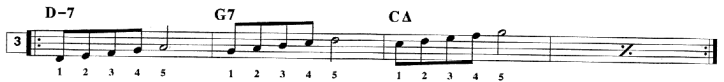
\includegraphics[width=0.8\linewidth]{scans251/major3.png}\item Used in \cref{minor1-1}
\newline\newline
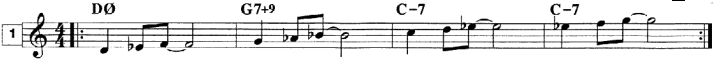
\includegraphics[width=0.8\linewidth]{scans251/minor1.png}\item Used in \cref{minor8-1}
\newline\newline
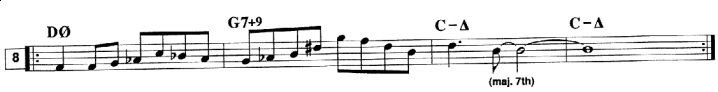
\includegraphics[width=0.8\linewidth]{scans251/minor8.png}
\end{itemize}

\end{document}
